\documentclass[a4paper]{article}
\usepackage{fullpage}
\oddsidemargin = -0.5in

\iffalse added for extra functionality \fi
\usepackage{booktabs}% http://ctan.org/pkg/booktabs
\newcommand{\tabitem}{~~\llap{\textbullet}~~}
\usepackage{graphicx,wrapfig,lipsum,mathtools}

\begin{document}

\section{Web small history}
	\subsection{Hypertext}
		\begin{itemize}
		\setlength{\itemsep}{-3pt}
		\item Vannever Bush invented hypertext as idea (without implementing it) in 1945
		\item hypertext was supposed to be a document system with links from document to document
		\item many scientific implementations 
		\end{itemize}
	\subsection{Web}
		\begin{itemize}
		\setlength{\itemsep}{-3pt}
		\item first to formulate idea of Web was Tim Berners-Lee
		\item idea was to have hypertext, that linked to other hypertext (very simple)
		\item TBL's dream was about the universal sharing of information
		\item if his dream is succesfull, the 'Web' becomes a {\bf realistic mirror} of society \\
		$\xrightarrow[]{}$ the web fits this description
	\end{itemize}
\section{Web \& Information Systems}
	\subsection{Information System design}
		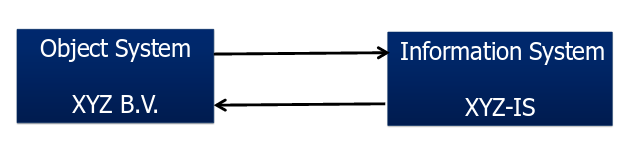
\includegraphics[width=300pt]{img/IS-Visualization.png}
		\begin{itemize}
		\setlength{\itemsep}{-3pt}
		\item mostly a mediator between {\bf System Object} and web
		\item requires knowledge about the System Object
		\item Web can be front- or back-end here
		\item if the Web is the front-end we call it \\{\bf Interface}
		\item databases in Web based {\bf IS} have to be fresh (new thing)
		\end{itemize}
	\subsection{Views on Web-Engineering}
		\subsubsection{WebML View}
			\begin{itemize}
			\setlength{\itemsep}{-3pt}
			\item interfaces meant for general public
			\item Web-IS are there to publish and maintain large amounts of data
			\end{itemize}
		\subsubsection{OOHDM View}
			Object-Oriented Hypermedia Design Method
			\begin{itemize}
			\setlength{\itemsep}{-3pt}
			\item Web brought {\bf Navigation} \& {\bf Operations} to IS
			\item Web-based IS were first good hypermedia applications
			\end{itemize}
		\subsubsection{Nielsen's View}
			\begin{itemize}
			\setlength{\itemsep}{-3pt}
			\item on Web only constant is {\bf change}
			\item a good navigation structure is the key to success
			\end{itemize}
	\newpage
	\subsection{Challenges}
		Our focus is on applications whos purpose is to publish and maintain large amounts of data.
		The {\bf Web-Browser} is the {\bf front-end}, the {\bf database} is the {\bf back-end}.
		This presents a few challenges:\\
		\begin{itemize}
		\setlength{\itemsep}{-3pt}
		\item What data do we have? {\bf Data structures}
		\item How do we organize the data for access? {\bf Navigation}
		\item How do we represent the data in access? {\bf Presentation(layout)}
		\item How do we do the back-end {\bf Database/repository management}
		\end{itemize}
	\subsection{Evolution of Web}
		The Evolution of the Web is not a managed process. Web 1.0 was meant to mainly
		show content, made by the site-owner. Web 2.0 went over to having content 
		generated and managed by the user of the site. Web 3.0 want to go over to 
		having "Semantic Web" where everything is tagged with meta-data and not 
		only readable by humans	but also by machines.
\section{Web Science}
	The Web is more than a software system. It is the biggest human artifact.
	The science of how it works is called Web Science.\\
	The Web can be viewed as a IS, where the System Object is society. It is important
	to take society in account and not only the web-technology, since sitew with the
	same technology (e.g. Wikipedia, MediaWiki) do not operate in the same way.\\\\
	\begin{tabular}{cc}
	\bf Science approach & \bf CS approach\\
	What does the Web do? & What should the Web do?\\
	\textbackslash & /\\
	\end{tabular}\\
	\begin{tabular}{cccc}
	&&&Together they make Web Science
	\end{tabular}\\
	The Web is a huge graph, where the Nodes are not static and are influenced by
	things outside of the graph.
\end{document}